\title{SDN Project Proposal}
\author{
        David Poliakoff \\
        David Ozog \\
}
\date{\today}

\documentclass[12pt]{article}
\usepackage{graphicx}
\usepackage{amsmath}
\newcommand{\HRule}{\rule{\linewidth}{0.3mm}}

\begin{document}
\maketitle
\centerline{\HRule}

%\begin{abstract}
%This is the paper's abstract \ldots
%\end{abstract}

\section*{Problem:}
\label{problem}
A great deal of flexibility is available within the SDN paradigm 
where there is a complete separation of the networking data plane from the control plane via
software abstractions.  One area that is left to be explored is how large-scale computational applications
can benefit from the control abstraction layers that SDN provides.
We believe that having the ability to reconfigure the network 
at application runtime can provide opportunity for optimizations that were 
previously not possible.  Furthermore, event counters and statistics
that are provided by OpenFlow switches could provide valuable
information for computational load balancing that is not available 
without such functionalities.   

An example of where this might be applicable is in applications that utilize
a Partitioned Global Address Space (PGAS), in which data is spread
across a distributed memory cluster in such a way that is abstracted from
the programmer.   For instance, the Global Arrays (GA) library provides a friendly
API for doing ``shared-memory style" programming on distributed memory commodity clusters.  
Specifically, one can easily do multi-dimensional matrix operations with a single call across
a collection of distributed machines.

Unfortunately, this complicates the issue of exploiting and optimizing data affinity
in many applications.  For example, the coupled cluster module of NWChem 
(built on PGAS/GA) performs large tensor contractions by splitting the global 
data space into smaller \textit{tiles}.  These tiles are gathered from ``relatively unknown" locations
in the PGAS and operated on locally with multiple iterations.  Unfortunately, it can be difficult for the application
to adapt to situations where data locality is poor.  With the power to measure 
network counters and reconfigure the network on the fly, problems such as this can 
potentially be alleviated.


\section*{Solution:}
\label{solution}
We propose to develop a simple synthetic application which performs a global operation on data
that is intentionally unoptimized for locality.  Because this problem can be difficult for application
programmers to solve based only on application-level information, we will design and develop a simple
%example application where SDN counters and re-configurations are used to improve data locality on the 
example application where SDN provided network traffic statistics will be used to reconfigure data to improve locality on the
fly.  The application will directly communicate with the controller process (or a proxy on its behalf)
to inform the application where data should be migrated in order to improve data locality for subsequent
operations and/or iterations.

\section*{Plan:}
\label{plan}
\begin{figure}[t]
\centerline{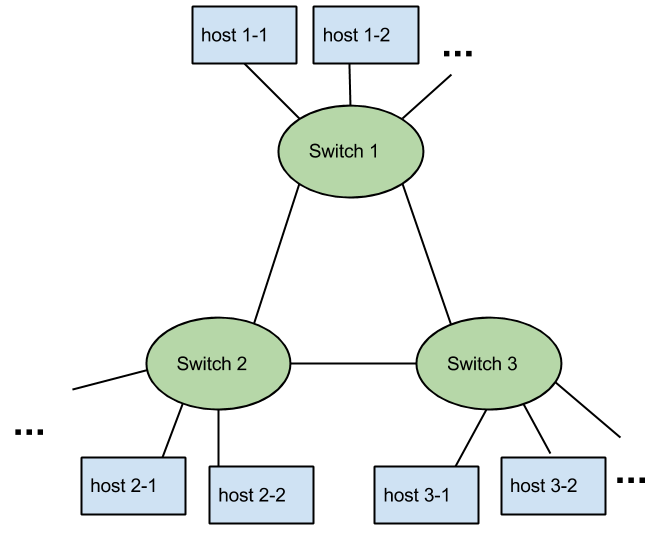
\includegraphics[width=3.0in]{img/topo.png}}
\caption{Simple topology for synthetic application}
\label{fig:topo}
\end{figure}
We will begin by constructing a small \texttt{mininet} configuration that mimics the UO testbed
that will soon be available (Figure~\ref{fig:topo}).  Then, we will work to correlate
inter-host traffic with application activity in the context of an application working in 
a global memory space.  If the multi-switch topology proves to be too difficult, we can 
start with a single switch and build upon that.  By constraining our simulated network to the
triangle switch, we hope to transition to the testbed environment as gracefully as possible.  However,
it will suffice to run our experiments within a \texttt{mininet} network only if need be.

Specifics of our approach still need to be worked out.  For instance, we are not sure if host-to-host
traffic statistics will be available in the OpenFlow switch flow tables (though we are pretty sure they
are...).  So it is yet to be determined whether our traffic matrix algorithm will be on host-to-host
traffic:

$
M = \bordermatrix{~ & h_1 & h_2 & h_3 & h_4 ... \cr
                  h_1 & 0 & a & b & c\cr
                  h_2 & a' & 0 & d & e\cr
                  h_3 & b' & d' & 0 & f\cr
                  h_4 & c' & e' & f' & 0\cr}
\vspace{5mm}
$
\\
\vspace{3mm}
\noindent or switch-to-switch traffic:

$
M = \bordermatrix{~ & s_1 & s_2 & s_3 \cr
                  s_1 & 0  & a & b \cr
                  s_2 & a' & 0 & c \cr
                  s_3 & b' & c' & 0 \cr}
$
\\
\vspace{3mm}

There is also the question of whether to work with per-flow counters, per-port counters, or both.

As a side note, we will be using a publicly viewable Git repository for holding version controlled code.

\vspace{10mm}

\section*{Timeline:}
\label{timeline}
\begin{center}
  \begin{tabular}{ l || c }
    \hline
    Date & Milestone \\ \hline \hline
    Week 4  & Simple mininet topology w/ counters per flow and per port \\ \hline
    Week 5  & Synthetic application in place with measurably poor data locality \\ \hline
    Week 6  & Structures for counters of relevant traffic data (traffic matrix) \\ \hline
    Week 7  & Analysis/algorithm for traffic data/migration decisions in place \\ \hline
    Week 8  & Data migration based on traffic analysis \\ \hline
    Week 9  & Performance comparison and evaluation \\ \hline
    Week 10 & Presentation, demonstration, discussion \\ 
    \hline
  \end{tabular}
\end{center}


\section*{Deliverables:}
\label{deriverables}
\begin{enumerate}
\item A synthetic application that performs a global operation (reduction) on data with poor locality
\item A controller / analyzer that collects relevant counter data and flow measurements and correlates them with application operations
\item A performance evaluation framework for this system
\item A presentation / demonstration of the project
\end{enumerate}



%\bibliographystyle{abbrv}
%\bibliography{SDN_Project_proposal}

\end{document}
This is never printed
